\documentclass[11pt,a4paper]{article}

\usepackage[spanish,es-noshorthands]{babel}
\usepackage[T1]{fontenc}
\usepackage[utf8]{inputenc}
\usepackage{lmodern}
\usepackage[a4paper,margin=2.4cm]{geometry}
\usepackage{graphicx}
\usepackage{booktabs}
\usepackage{array}
\usepackage{hyperref}
\usepackage{xcolor}
\usepackage{float}
\usepackage{caption}

\hypersetup{
    colorlinks=true,
    linkcolor=blue!60!black,
    urlcolor=blue!60!black
}

\title{Avance de Investigacion:\\ Exploracion sobre \texttt{Agent7250} y siguiente intervencion distinta}
\author{Proyecto EMG Prosthesis TD3}
\date{25 de marzo de 2026}

\begin{document}
\maketitle

\section{Estado de partida}

El benchmark operativo del proyecto sigue siendo \texttt{Agent7250}, obtenido en la corrida valida de \texttt{8000} episodios posterior al fix del simulador. La meta de esta fase no fue ``hacer que aprenda'' desde cero, sino intentar mejorar el compromiso entre tracking, esfuerzo de control y agresividad residual, sin tocar:

\begin{itemize}
\item observacion \texttt{markov52},
\item reward \texttt{trackingMseActionRateReward},
\item arquitectura TD3 feedforward,
\item cuantizacion y remapeo efectivo del actuador.
\end{itemize}

\begin{table}[H]
\centering
\caption{Benchmark operativo congelado: \texttt{Agent7250}}
\begin{tabular}{lr}
\toprule
Metrica & Valor \\
\midrule
\texttt{trackingMSE} & 0.043045 \\
\texttt{trackingMAE} & 0.160336 \\
\texttt{actionL2} & 0.596444 \\
\texttt{saturationFraction} & 0.392086 \\
\texttt{deltaActionL2} & 0.321385 \\
\texttt{absPWM mean} & 178.288566 \\
\bottomrule
\end{tabular}
\end{table}

\section{Idea anterior: continuacion de \texttt{Agent7250} con menor exploracion}

\subsection{Por que se intento}

El benchmark ya seguia bien la referencia, pero seguia siendo relativamente agresivo. La idea fue continuar el entrenamiento del propio \texttt{Agent7250} con menos ruido de exploracion, en vez de cambiar reward o crear un agente nuevo. La hipotesis era que, si la politica ya estaba en una buena region del espacio de parametros, una continuacion con ruido menor podia preservar tracking y reducir saturacion.

\subsection{Que se hizo}

Se implemento un flujo de \emph{resume training} con reaplicacion real del ruido de exploracion al checkpoint cargado. Sobre esa base se corrio un barrido sobre \texttt{explorationStd} y \texttt{explorationStdMin}, manteniendo fijo el resto del baseline.

La mejor combinacion auditada fue:

\begin{itemize}
\item \texttt{explorationStd = 0.05}
\item \texttt{explorationStdMin = 0.005}
\item \texttt{explorationStdDecayRate = 1e-4}
\item mejor checkpoint: \texttt{Agent1100}
\end{itemize}

\begin{table}[H]
\centering
\caption{Mejor resultado auditado de la continuacion con menor exploracion}
\begin{tabular}{lr}
\toprule
Metrica & Valor \\
\midrule
\texttt{trackingMSE} & 0.044022 \\
\texttt{trackingMAE} & 0.163450 \\
\texttt{actionL2} & 0.577940 \\
\texttt{saturationFraction} & 0.352710 \\
\texttt{deltaActionL2} & 0.191540 \\
\bottomrule
\end{tabular}
\end{table}

La lectura fue clara: el tracking empeoro poco, la saturacion bajo alrededor de un 10\% y \texttt{deltaActionL2} cayo mucho, pero \texttt{actionL2} no bajo lo suficiente para cumplir la \texttt{ConditionB}. Como politica ``mas suave'' fue interesante; como reemplazo del benchmark, no.

\subsection{Test visual del mejor candidato}

Se corrio un test completo de 50 simulaciones sobre ese \texttt{Agent1100}. El resultado agregado fue:

\begin{table}[H]
\centering
\caption{Test visual de 50 simulaciones del mejor candidato de baja exploracion}
\begin{tabular}{lr}
\toprule
Metrica & Valor \\
\midrule
\texttt{trackingMSE} & 0.047900 \\
\texttt{trackingMAE} & 0.172100 \\
\texttt{actionL2} & 0.530600 \\
\texttt{saturationFraction} & 0.337700 \\
\texttt{deltaActionL2} & 0.275200 \\
\texttt{absPWM mean} & 162.876400 \\
\bottomrule
\end{tabular}
\end{table}

\begin{figure}[H]
\centering
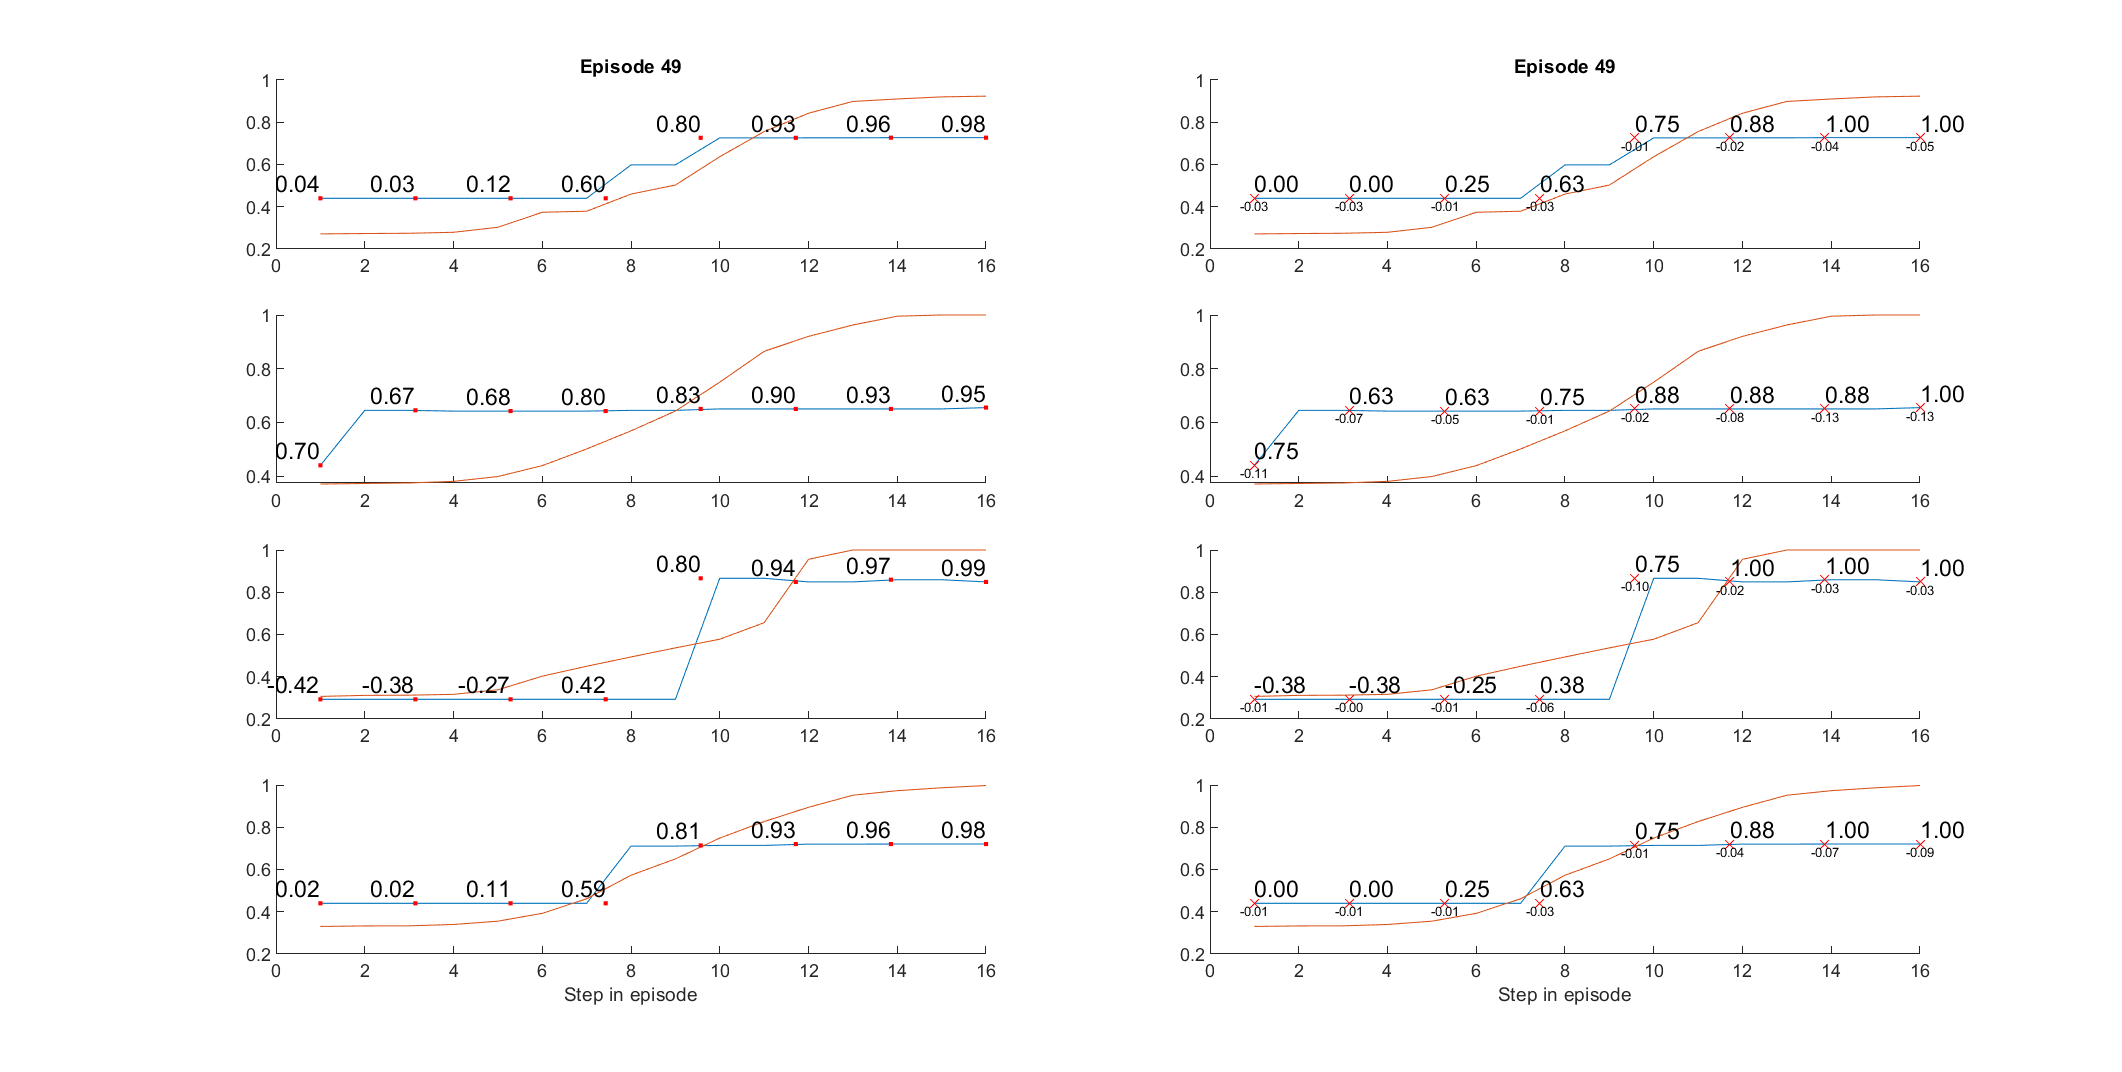
\includegraphics[width=0.88\linewidth]{figures/test_episode_49_agent1100_low_exploration.png}
\caption{Ejemplo visual del test del mejor candidato de baja exploracion. La politica es mas suave que el benchmark, pero el tracking cae demasiado para reemplazar a \texttt{Agent7250}.}
\end{figure}

\section{Idea actual cerrada: exploracion \textit{threshold-aware}}

\subsection{Por que surgio}

Revisando el comportamiento real del repo aparecio un hecho importante:

\begin{itemize}
\item \texttt{actionCommandActivationThreshold = 0.05}
\item el primer nivel no nulo cuantizado es \texttt{64/255 \textasciitilde{} 0.251}
\end{itemize}

Eso significa que una accion continua apenas por encima del umbral ya salta al primer comando fisicamente efectivo del actuador. La exploracion gaussiana no actua entonces sobre una planta suave, sino sobre una interfaz con una discontinuidad real.

La hipotesis fue que un barrido fino alrededor de esa discontinuidad podia conservar tracking y bajar agresividad, sin tocar reward, observacion ni arquitectura.

\subsection{Protocolo aplicado}

Se implemento un \emph{launcher} por etapas:

\begin{enumerate}
\item \texttt{stage1}: sweep fino de \texttt{explorationStd} alrededor del umbral.
\item \texttt{stage2}: ablation de \texttt{explorationStdDecayRate}.
\item \texttt{stage3}: prueba unica con \texttt{ResetExperienceBufferBeforeTraining = true}.
\end{enumerate}

\subsection{Resultados}

\begin{table}[H]
\centering
\caption{Resumen de la ruta \textit{threshold-aware}}
\begin{tabular}{>{\raggedright\arraybackslash}p{2.3cm}ccccc}
\toprule
Etapa & trackingMSE & actionL2 & saturationFraction & deltaActionL2 & Veredicto \\
\midrule
Stage 1 mejor (\texttt{0.05 / 0.005 / 1e-4}) & 0.044022 & 0.577940 & 0.352710 & 0.191540 & Casi-acierto \\
Stage 2 mejor (\texttt{decay = 1e-4}) & 0.044022 & 0.577940 & 0.352710 & 0.191540 & Sin mejora nueva \\
Stage 2 (\texttt{decay = 0}) & 0.047686 & 0.587490 & 0.361530 & 0.207090 & Peor tracking \\
Stage 2 (\texttt{decay = 5e-5}) & 0.047702 & 0.716040 & 0.536630 & 0.176300 & Mucho mas agresivo \\
Stage 3 (\texttt{reset = true}) & 0.044022 & 0.577940 & 0.352710 & 0.191540 & Repite stage 1 \\
\bottomrule
\end{tabular}
\end{table}

\begin{figure}[H]
\centering
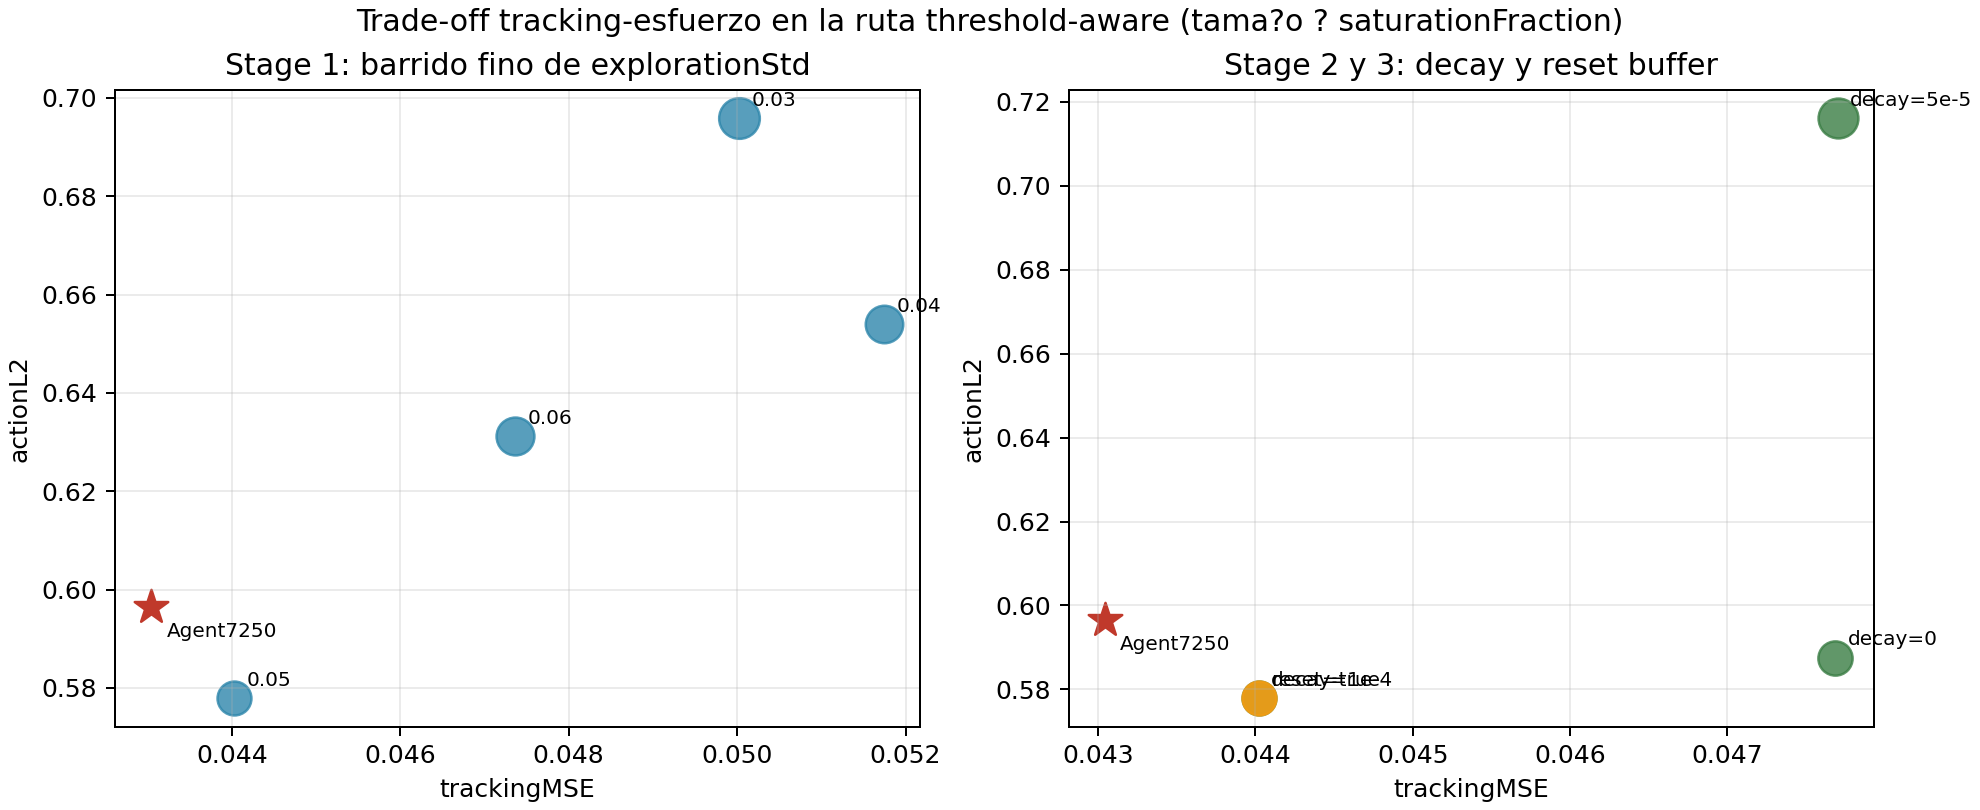
\includegraphics[width=\linewidth]{figures/threshold_exploration_tradeoff_20260325.png}
\caption{Trade-off tracking-esfuerzo de la ruta \textit{threshold-aware}. El tamano del marcador es proporcional a \texttt{saturationFraction}. El benchmark \texttt{Agent7250} aparece en rojo.}
\end{figure}

\subsection{Lectura tecnica}

La ruta \textit{threshold-aware} fue metodologicamente correcta y valiosa para cerrar una hipotesis concreta del repo. Sin embargo:

\begin{itemize}
\item el mejor punto siguio siendo el mismo casi-acierto ya visto con baja exploracion,
\item bajar mas el ruido no ayudo,
\item cambiar el decaimiento no abrio una mejora nueva,
\item resetear el \emph{replay buffer} tampoco produjo una ventaja observable.
\end{itemize}

En otras palabras, esta linea si mejoro suavidad, pero no produjo una politica nueva capaz de reemplazar a \texttt{Agent7250}.

\section{Nueva intervencion ejecutada: piloto de accion continua alineada al actuador}

\subsection{Por que se intento}

La lectura que dejo la fase anterior fue que el cuello de botella ya no parecia ser ``cuanto ruido meter'', sino la desalineacion entre:

\begin{itemize}
\item la accion continua que emite el actor en \texttt{[-1,1]},
\item el umbral de activacion \texttt{0.05},
\item y la cuantizacion posterior a niveles PWM efectivos.
\end{itemize}

Sobre esa base se implemento una nueva interfaz de accion llamada \texttt{alignedContinuousWarp}. La idea era sencilla: antes del remapeo final al actuador, la magnitud continua del actor se deformaba para aproximarla a los niveles fisicamente utiles del sistema. Con ello se queria reducir el espacio ``muerto'' entre accion continua y accion efectiva, sin tocar reward, observacion ni arquitectura.

\subsection{Protocolo aplicado}

El piloto mantuvo fijo:

\begin{itemize}
\item checkpoint base: \texttt{Agent7250},
\item observacion \texttt{markov52},
\item reward \texttt{trackingMseActionRateReward},
\item TD3 feedforward,
\item exploracion \texttt{0.05 / 0.005 / 1e-4},
\item \texttt{1500} episodios adicionales con guardado cada \texttt{50}.
\end{itemize}

La warp introducida en la interfaz del entorno uso:

\begin{itemize}
\item \texttt{deadzone = 0.05},
\item niveles de salida \texttt{[64 96 128 160 192 224 255] / 255},
\item conservacion del signo de la accion original.
\end{itemize}

El entrenamiento termino correctamente en la carpeta:

\begin{itemize}
\item \texttt{Agentes/agent7250\_aligned\_action\_pilot/26-03-25 10 44 29/training\_run/26-03-25 10 44 38}
\end{itemize}

Sin embargo, la auditoria integrada no cerro bien el resumen consolidado. Para no perder la corrida, se reconstruyo manualmente la auditoria completa en:

\begin{itemize}
\item \texttt{Agentes/agent7250\_aligned\_action\_pilot/26-03-25 10 44 29/audit\_rebuilt}
\end{itemize}

\subsection{Resultado auditado}

La fase rapida ya mostraba un patron claro: podia aparecer un \texttt{trackingMSE} atractivo, pero a costa de mucho mas borde y mucho mas esfuerzo. La fase completa confirmo que la mejor politica del piloto fue \texttt{Agent1450}, y que aun asi quedaba rechazada.

\begin{table}[H]
\centering
\caption{Auditoria reconstruida del piloto \texttt{alignedContinuousWarp}}
\begin{tabular}{lrrrr}
\toprule
Checkpoint & trackingMSE & actionL2 & saturationFraction & deltaActionL2 \\
\midrule
\texttt{Agent1450} & 0.044561 & 0.847337 & 0.676780 & 0.300599 \\
\texttt{Agent1350} & 0.047558 & 0.824998 & 0.645571 & 0.431538 \\
\texttt{Agent7250} benchmark & 0.043045 & 0.596444 & 0.392086 & 0.321385 \\
\bottomrule
\end{tabular}
\end{table}

Frente al benchmark, el mejor checkpoint del piloto:

\begin{itemize}
\item empeora \texttt{trackingMSE} en aproximadamente \texttt{+3.5\%},
\item empeora \texttt{actionL2} en aproximadamente \texttt{+42.1\%},
\item empeora \texttt{saturationFraction} en aproximadamente \texttt{+72.6\%},
\item solo mejora un poco \texttt{deltaActionL2}.
\end{itemize}

Por tanto, el piloto no paso ni el filtro practico previo al test visual. No se genero \texttt{visual\_test} final porque la politica ya quedaba claramente fuera del compromiso minimo exigido.

\begin{figure}[H]
\centering
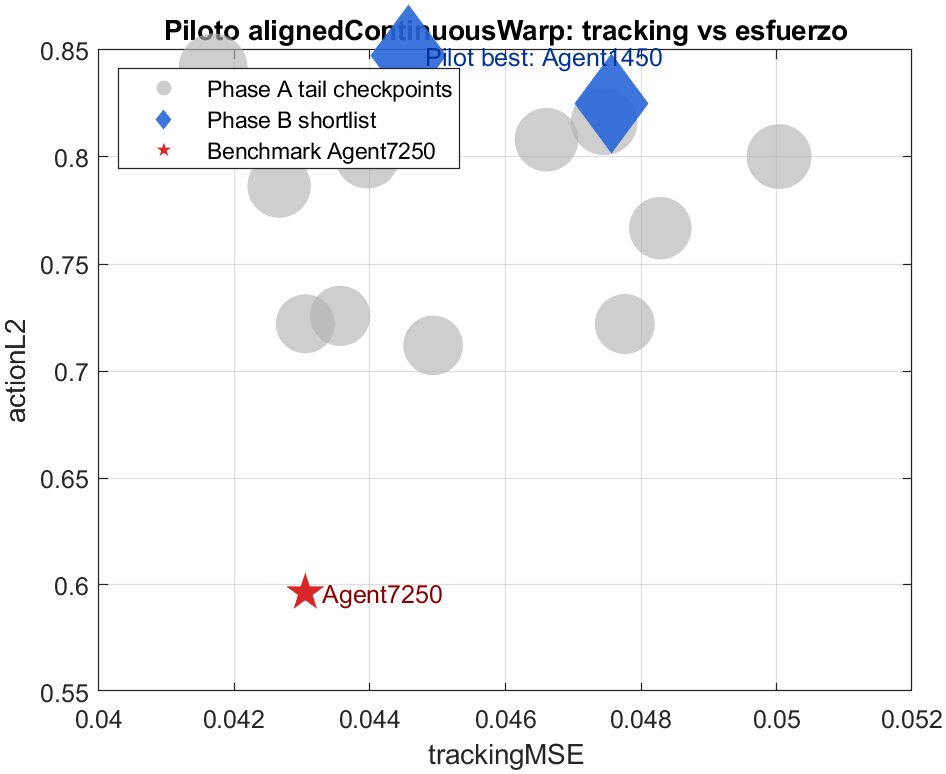
\includegraphics[width=\linewidth]{figures/aligned_action_pilot_tradeoff_20260325.png}
\caption{Trade-off de la cola auditada del piloto \texttt{alignedContinuousWarp}. El tamano del marcador es proporcional a \texttt{saturationFraction}. El benchmark \texttt{Agent7250} sigue en una region mucho mas razonable del compromiso.}
\end{figure}

\subsection{Que enseno el logging nuevo}

Esta intervencion si fue valiosa como experimento de diagnostico porque el nuevo logging mostro por que la idea fallaba. Sobre toda la corrida de entrenamiento:

\begin{itemize}
\item \texttt{trackingMSE mean} del run: \texttt{0.045688},
\item \texttt{actionL2 mean}: \texttt{0.751889},
\item \texttt{saturationFraction mean}: \texttt{0.519368},
\item \texttt{deltaActionL2 mean}: \texttt{0.414207},
\item \texttt{rawToWarpedActionErrorMean}: \texttt{0.043347},
\item fraccion cruda en la zona \texttt{0.05 <= |u| < 64/255}: \texttt{0.065893}.
\end{itemize}

En el mejor checkpoint auditado (\texttt{Agent1450}), la informacion por bins deja el patron todavia mas claro:

\begin{itemize}
\item \texttt{rawToWarpedActionErrorMean}: \texttt{0.027231},
\item \texttt{rawDeadzoneToFirstLevelFractionMean}: \texttt{0.038733},
\item fraccion en \texttt{effectiveAction = +1.0}: \texttt{0.621576},
\item fraccion en \texttt{effectiveAction = 0}: \texttt{0.005055}.
\end{itemize}

Es decir, la warp no ayudo a usar mejor la zona intermedia. En la practica, el agente aprendio a explotar mas agresivamente el borde superior positivo del actuador.

\begin{figure}[H]
\centering
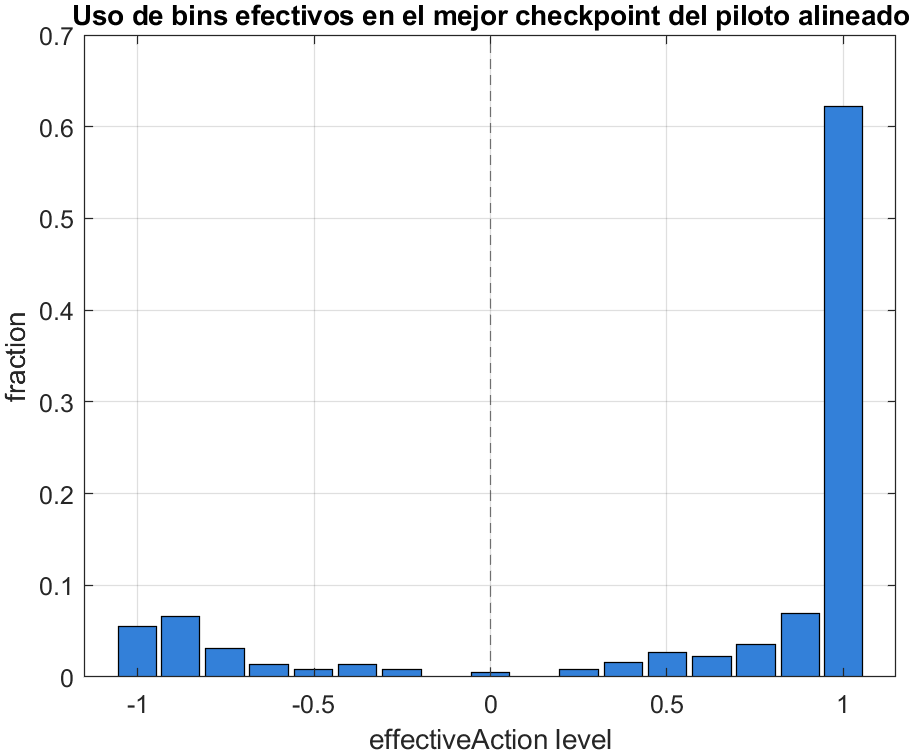
\includegraphics[width=\linewidth]{figures/aligned_action_pilot_bin_usage_20260325.png}
\caption{Uso de niveles efectivos en el mejor checkpoint del piloto alineado. La masa se desplaza con fuerza al bin \texttt{+1.0}, lo que explica el aumento de saturacion y esfuerzo.}
\end{figure}

\subsection{Lectura tecnica}

La hipotesis de trabajo era razonable: si el problema estaba en la desalineacion entre accion continua y actuador cuantizado, una warp fija podia acercar ambos mundos. Lo que mostro el experimento es que, al menos en esta forma, la warp fija no regulariza el control, sino que abre una ruta mas directa para colapsar a bins altos.

Eso cambia la lectura de la linea:

\begin{itemize}
\item la desalineacion actor-actuador sigue siendo un problema plausible,
\item pero una deformacion fija en la interfaz del entorno no lo resuelve,
\item y de hecho puede amplificar la tendencia a saturar.
\end{itemize}

\section{Conclusion tecnica actualizada de la fase}

A esta altura, tres lineas distintas ya quedaron suficientemente exploradas:

\begin{itemize}
\item continuacion con baja exploracion,
\item exploracion \textit{threshold-aware},
\item piloto de accion continua alineada con warp fija.
\end{itemize}

Las tres dejaron aprendizaje util, pero ninguna reemplazo al benchmark \texttt{Agent7250}. La lectura consolidada queda asi:

\begin{itemize}
\item bajar un poco la exploracion ayuda a suavizar, pero no alcanza para ganar en tracking y control a la vez;
\item seguir exprimiendo exploracion gaussiana no abre una mejora nueva;
\item alinear la interfaz de accion con una warp fija tampoco funciona, porque la politica tiende a colapsar a bins altos;
\item el benchmark \texttt{Agent7250} sigue siendo el punto operativo mas solido del proyecto.
\end{itemize}

\section{Siguiente intervencion distinta recomendada}

La siguiente intervencion ya no deberia ser:

\begin{itemize}
\item otra reward nueva,
\item otro sweep de exploracion,
\item ni otra warp fija en la interfaz del entorno.
\end{itemize}

Si se decide seguir trabajando la cuestion del actuador, la siguiente idea debe ser mas estructural: no una deformacion fija impuesta fuera de la politica, sino una parametrizacion de accion o una restriccion de uso de bins que este acoplada al aprendizaje y no incentive el colapso al nivel maximo. En otras palabras, la direccion nueva ya no es ``explorar mejor'' ni ``warpear mejor'', sino disenar una salida de politica que represente de forma mas honesta el actuador cuantizado.

\section{Mensaje final de avance}

El documento de avance puede ampliarse ya con una conclusion fuerte y defendible:

\begin{itemize}
\item \texttt{Agent7250} sigue siendo el benchmark operativo vigente;
\item la rama de baja exploracion dejo un candidato mas suave, pero no un nuevo baseline;
\item la rama \textit{threshold-aware} cerro la hipotesis de exploracion alrededor del umbral;
\item el piloto \texttt{alignedContinuousWarp} mostro que una warp fija puede empeorar el compromiso al colapsar a bins altos;
\item la siguiente fase debe abandonar la exploracion como variable principal y replantear la interfaz de accion desde una representacion mas estructural.
\end{itemize}

\end{document}
